\documentclass[letterpaper, 10 pt, conference]{ieeeconf}

\IEEEoverridecommandlockouts
\overrideIEEEmargins

\usepackage{graphics}
\usepackage{epsfig} 
\usepackage{listings} 
\lstset{language=C}

\newenvironment{mylisting}
{~\par~\begin{list}{}{\setlength{\leftmargin}{1em}}\item\scriptsize\bfseries}
{\end{list}~\par}


\title{\LARGE \bf
Expert System Design for an Autonomous Driver Evaluation System
}

\author{}
\author{Kemal~Kaplan and H.~Levent~Ak{\i}n, \textit{Senior Member, IEEE} \thanks{Manuscript received \today.}\thanks{Kemal Kaplan, and H.~Levent Ak{\i}n  are with the Department of Computer Engineering, Bo{\u g}azi{\c c}i University, 34342, Bebek, \.{I}stanbul, Turkey. (e-mail~:~kaplanke@boun.edu.tr; akin@boun.edu.tr)}}

\begin{document}
\maketitle
\thispagestyle{empty}
\pagestyle{empty}


%%%%%%%%%%%%%%%%%%%%%%%%%%%%%%%%%%%%%%%%%%%%%%%%%%%%%%%%%%%%%%%%%%%%%%%%%%%%%%%%
\begin{abstract}
In this paper, two expert system implementations for the Automatic Driver Evaluation System (ADES) Project are introduced. These expert systems are used for deciding whether a driver violates the traffic rules or not, according to the facts derived from the data acquired by the sensors. Sample scenarios are executed in a highly realistic simulation environment. The advantages and shortcomings of both approaches are discussed. 
\end{abstract}

%%%%%%%%%%%%%%%%%%%%%%%%%%%%%%%%%%%%%%%%%%%%%%%%%%%%%%%%%%%%%%%%%%%%%%%%%%%%%%%%
\section{INTRODUCTION}
Traffic accidents are one of the main causes of death and economic loss in most of the developed countries. According to the Road Safety Action Program of European Commission, more than one million accidents a year cause more than 40 000 deaths and nearly two million injuries on the roads. On the other side, the direct and indirect cost has been estimated at 160 billion Euros \cite{Eu01}. Nearly all of these accidents are caused by driver mistakes. 

The ADES project is a framework for developing real time on-vehicle applications for detecting the traffic violations committed by the drivers. The project has three main modules. The first module acquires raw data using different sensors like camera, RF reader or GPS. The second module processes the data acquired by these sensors. The final module, which is the inference engine, tries to detect the violations by using this information. The inference engine should contain a reasoning mechanism, which is usually an expert system or a mixture of expert systems, for deciding and justifying the violations. Any expert system proposed for ADES project should be able to use the information gathered from the environment. This information should be processed considering the traffic rules. The proposed expert system should also handle the uncertainty due to the inaccuracy of the sensors or the misleading data processing results. The overall structure of the ADES project is shown in Figure \ref{fig:sys}.

\begin{figure}[thb]
      \centering
      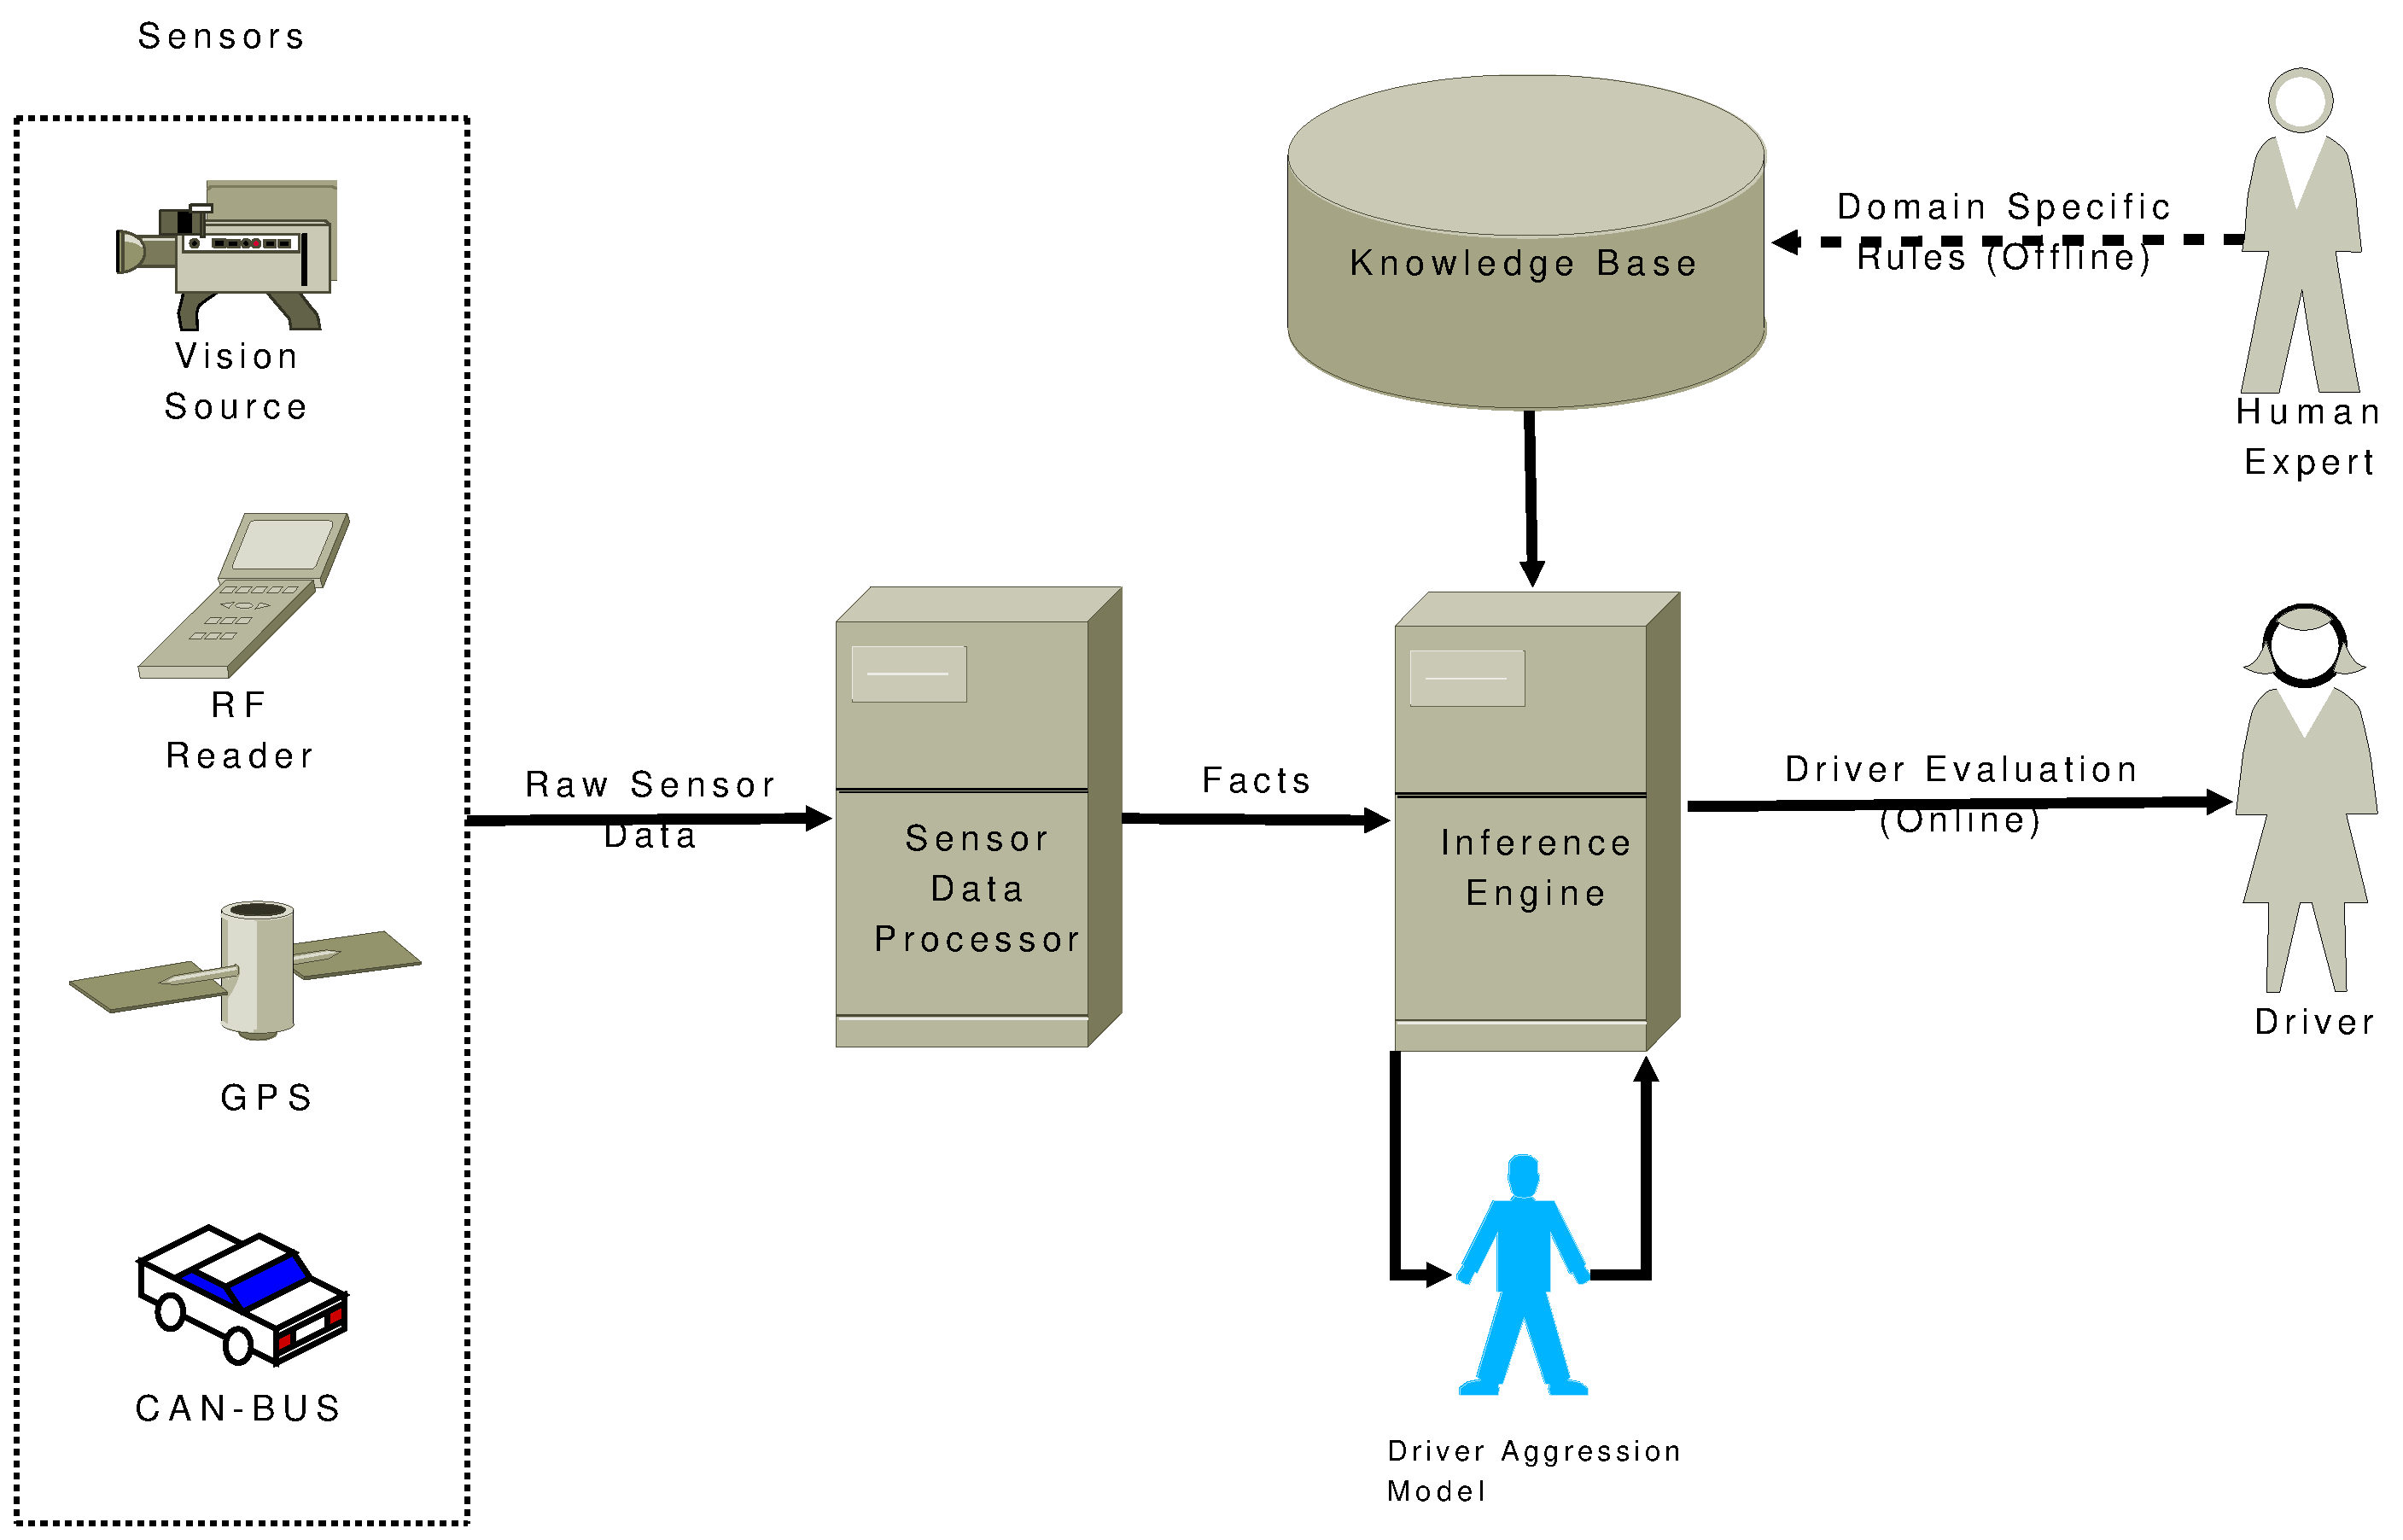
\includegraphics[scale=0.16]{img/sys3}
      \caption{The overall structure of the ADES project.}
      \label{fig:sys}
\end{figure}

Although autonomous driver evaluation is a new research area, expert systems are widely used for similar purposes such as autonomous driving. Sukthankar \textit{et al}  ~\cite{Sukthankar97} presented a distributed solution, which consists of a collection of reasoning objects that vote upon a set of possible actions for dealing with the complexity of tactical reasoning. Rosa \textit{et al} ~\cite{Rosa97} implemented a fuzzy expert system to organize traffic regulations in a town area. Al-Shihabi \textit{et al} ~\cite{Shihabi01}  proposed a framework for modeling driver behavior with perception, emotions, decision-making, and the decision-implementation units formed of fuzzy variables and if-then rules.  Gao and Zhou  ~\cite{Gao05} developed a fuzzy rule based control strategy selection approach for mobile navigation which utilizes fuzzy reasoning Petri nets for system modeling and parallel reasoning. Lattner \textit{et al} ~\cite{Lattner05} introduced a knowledge-based approach to behavior decision for intelligent vehicles which uses qualitative representation of the information perceived by the sensors. Long \textit{et al} ~\cite{Long07} presented a review of software platforms for autonomous vehicles and their artificial intelligence development capabilities. Ferguson \textit{et al} ~\cite{Ferguson08} presented a reasoning framework, which consists of the mission, behavioral, and motion planning components performing reasoning for an autonomous vehicle navigating through urban environments. Vacek \textit{et al} ~\cite{Vacek07} used case-based reasoning in order to predict the progress of the current situation and to select the appropriate behavior. DuToit \textit{et al} ~\cite{Dutoit08} described a finite state machine model to manage the complexity of the situational reasoning subsystem which recognizes the current situation to impose the correct traffic rules.

In this study we consider two different expert systems namely a probabilistic \textit{Prolog} based and Bayesian Network based, to manage the challenging task of real-time driver evaluation. The proposed systems can accept the predefined rules from the human experts, use the information provided by the outside world for reasoning, and handle the uncertainty by considering the probabilities of the accuracy of this information.

The organization of the rest of the paper is as follows. \textit{Prolog} and Bayesian Network based expert systems are discussed in Section \ref{sec:KR}. In Section \ref{sec:proposed} the proposed approach is explained. Experimental evaluation of the proposed expert systems in a highly realistic simulation environment is given in Section \ref{sec:experimental}. Discusion of the results and the conclusions are given in Section \ref{sec:conc}. 


\section{Knowledge Representation Approaches}
\label{sec:KR}

Expert systems may use different knowledge representation approaches. Here we consider two of them, namely \textit{Prolog} based and Bayesian Networks based.

\subsection{\textit{Prolog} Programming Language}

\textit{Prolog} is a logic programming language. It is suitable for solving problems which contains objects and relations between these objects. The relations defined over the variables are called the \textit{rules}. On the other hand, the \textit{facts} are the means of stating that relations that exist between the objects. Therefore, the relations of the facts only contain atoms \cite{bratko2001\textit{Prolog}, sterling1994art}. The power of \textit{Prolog} comes from three major features of the language which are rule-based programming, built-in pattern matching, and backtracking execution. Pattern matching and backtracking features provide automatic control of the flow in the program which make it possible to realize many types of expert systems \cite{merritt1989building}.

There are a few applications of \textit{Prolog} in autonomous vehicle researches. Brunet \textit{et al} used a \textit{Prolog} based programming language for developing a multi-agent architecture for an autonomous vehicle driver model ~\cite{brunet95}. Piaggio \textit{et al} used a \textit{Prolog} based application to implement the symbolic component of their real time autonomous motion planning approach, which is responsible for high level planning ~\cite{Piaggio00}.

\subsection{Belief Networks}

A belief network (BN) is an acyclic graph used for modeling the uncertainty in a domain \cite{pearl1986fusion}. The nodes of the graph are random values and the arcs are conditional dependencies between these variables. BNs are reasoning tools based on probability. Although it is possible to design multiply-connected (or cyclic) BNs, probabilistic inference using this type of networks is NP-hard \cite{cooper1990computational}.

BNs have been studied in autonomous driving or driver assistant systems for more than a decade. The idea behind the time dependent dynamic Bayesian networks is quite similar with Markovian Models and Kalman Filters. In 1995, Forbes \textit{et al} \cite{forbes1995batmobile} proposed the \textit{Bayesian Automated Taxi (BATmobile)} which is a decision-theoretic architecture using dynamic probabilistic networks for autonomous driving. The BATmobile used dynamic Bayesian networks where the states of the variables are also considered in the decision process. In addition to having Markovian property, the proposed network also modifies its internal structure by adding or removing the time slices. In 2002, Ross \textit{et al} \cite{ross2002mobile} described a distributed information fusion system based on hierarchical BNs using D'Agent mobile agent system. In the proposed system the structure of the BN can be rearranged according to the gathered information. Kumagai \textit{et al} \cite{kumagai2003prediction} also used dynamic BN to predict the driver's stopping behavior. The structure and the parameters of the network are calculated by using the pedal strokes and the speed of the vehicle during the learning phase. Dagli \textit{et al} \cite{dagli2010action} also used a similar technique for predicting the lane departure behaviors of the drivers. In 2008, Petrovskaya \textit{et al} \cite{petrovskaya2008model} used a dynamic BN model for tracking the vehicles during DARPA urban challenge. The positions and the orientations of the vehicles are used for predicting the future location of the vehicles.

%%%%%%%%%%%%%%%%%%%%%%%%%%%%%%%%%%%%%%%%%%%%%%%%%%%%%%%%%%%%%%%%%%%%%%%%%%%%%%%%
\section{PROPOSED APPROACH}
\label{sec:proposed}

The targeted traffic rules considered in this study, the sample traffic signs related with these regulations, and the possible inputs to the system for assertion, retraction, and evaluation of these rules are given in Table \ref{viol}. Different combinations of these inputs can be used for different violations. 

\begin{table}[!ht]
\caption{Targeted traffic violations.}
\centering
{\scriptsize
\begin{tabular}{|r|r|c|}
\hline
&&\\
No Turn Left & 
\includegraphics[scale=0.25]{img/noleft} & Sign Detection,\\
&&\\
\cline{1-2}
&&\\
No Turn Right & 
\includegraphics[scale=0.25]{img/noright} & RFID Detection,\\
&&\\
\cline{1-2}
&&\\
 No U Turn & 
\includegraphics[scale=0.25]{img/nouturn} & GPS/GIS Information,\\
&&\\
\cline{1-2}
&&\\
No Entrance & 
\includegraphics[scale=0.25]{img/noenter} & Vehicle Speed,\\
&&\\
\cline{1-2}
&&\\
Speed Limit & 
\includegraphics[scale=0.25]{img/speedlimit} & Steering Angle, \\
&&\\
\cline{1-2}
&&\\
No Overtaking & 
\includegraphics[scale=0.25]{img/overtake} & Lane Detection,\\
&&\\
\cline{1-2}
&&\\
Traffic Lights & 
\includegraphics[scale=0.25]{img/trafficligt} &  Time Elapsed\\
&&\\
\cline{1-2}
&&\\
Emergency Lane &  
\includegraphics[scale=0.25]{img/eds} & \\
&&\\
\hline
\end{tabular}  
}
\label{viol}
\end{table}

Here for the sake of simplicity we present only two kind of traffic violations which are directional restrictions and speed limits. In addition, the inputs are the detected traffic signs, RFID readings and speed of the vehicle. Other inputs like GPS information, road lanes, or steering angle are not considered in the following sections. However, the design of the proposed expert systems allows the human expert to insert new rules without changing the implementation of the expert system.

\subsection{ADES Interface for Expert Systems}

In order to allow implementing generic expert systems  we defined an interface for integrating various expert system implementations into the ADES project as shown in Fig. \ref{fig:interface}. 

\begin{figure}[!ht]
      \centering

\begin{mylisting}

\begin{verbatim}
public interface ExpertSystems
        {
            string init(params object[] esParams);
            string assertFact(params object[] esParams);
            string retractFact(params object[] esParams);
            string[] query(params object[] esParams);
            void setThreshold(double threshold);
            double getThreshold();
        }
\end{verbatim}
\end{mylisting}
      \caption{ADES Interface for Expert Systems}
      \label{fig:interface}
\end{figure}

The $init$ function initializes the expert system with various parameters. The $assertFact$ function provides the high level information to the expert system. This information is formed by processing the data acquired from different sensors. The $retractFact$ function is used when a previously introduced information is invalidated. However, the expert systems are free to retract their facts according to their internal operations. The $query$ function is the main procedure triggered right after a fact is asserted or retracted. This function is expected to return the kind of violation and its probability if there is a traffic violation. Finally, the $setThreshold$ and $getThreshold$ functions are used for arranging the threshold level of the expert system for deciding a violation.


\subsection{Probabilistic \textit{Prolog} Based Expert System}

In the ADES project and many other real life problems, the relations between the objects are not always very clear. Therefore, the expert system should also consider the uncertainties associated with the supplied data. Therefore we used a modified version of \textit{Prolog} language which allows assignment of probabilities to the facts. There are also other \textit{Prolog} implementations available where the probability processing extensions can be consulted as libraries without changing the engine itself \cite{de2007problog}. We also introduce another improvement which is called \textit{time decaying facts}. We assign time limits for the facts with a second parameter whenever necessary. This is an important feature since the duration of some local regulations (like directional restrictions) can be determined according to the speed of the vehicle.

The \textit{Prolog} rule and sample facts for speed limit violation detection are as given in Fig. \ref{fig:rules}.

\begin{figure}[thb]
      \centering

\begin{mylisting}

\begin{verbatim}
%rule declaration
violation(V,A,P) :- velocity_exceeds(S),
                    sign_detected(V,L),
                    S>L,
                    atom_chars(S,L1),
                    append(L1,[95],L2),
                    atom_chars(L,L3),
                    append(L2,L3,L4),
                    atom_chars(A,L4),
                    prob(P).
%sample facts asserted by sensor systems 
velocity_exceeds(50)
"0.9::sign_detected(speed_limit,50)"
\end{verbatim}
\end{mylisting}

      \caption{Rules and Facts for Speed Limit}
      \label{fig:rules}
\end{figure}

The speed limit violation is decided according to the speed of the vehicle and the detection of the traffic sign for a particular speed limit. The violation predicate returns the final probability of the traffic violation if it can unify the $V$ parameter. The first sample fact in Fig. \ref{fig:rules}  states that the vehicle exceeds 50 km/h with a probability of $1$. The second sample fact is asserted for a speed limit sign for 50 km/h is detected with a probability of $0.9$.

The \textit{Prolog} rule and sample facts for directional restrictions are as given in Fig. \ref{fig:directional}.

\begin{figure}[thb]
      \centering
\begin{mylisting}

\begin{verbatim}
%rule declaration
violation(V,A,P) :- sign_detected(V),
                    rfid_detected(pre,V),
                    rfid_detected(post,V),
                    A is "N/A",
                    prob(P).
%sample facts asserted by sensor systems
"0.9::sign_detected(no_turn_left)"
"0.9::sign_detected(no_turn_right)"
"0.9::sign_detected(no_uturn)"
"0.9::30::rfid_detected(pre,no_turn_left)"
"0.9::30::rfid_detected(pre,no_turn_right)"
"0.9::30::rfid_detected(pre,no_uturn)"
"0.9::30::rfid_detected(post,no_turn_left)"
"0.9::30::rfid_detected(post,no_turn_right)"
"0.9::30::rfid_detected(post,no_uturn)"
\end{verbatim}
\end{mylisting}
      \caption{Rules and Facts for Directional Restrictions}
      \label{fig:directional}
\end{figure}

This violation occurs when the vehicle detects a no turning sign for left, right or U turn. In addition to the sign, the RFID tag which is assigned to that sign should be sensed. In addition to the speed limits signs, an additional confirmation RFID tag should also be sensed to complete the unification of the violation rule. The $V$ parameter gives the name of the violation and the $P$ parameter gives the probability of the violation. The sample rules are similar to the previous ones where $0.9$ presents the accuracy of the information. The sample facts about the RFID detections benefit from both improvements of our \textit{Prolog} implementation. The probability of this reading is $0.9$ and this fact will be removed from the system after $30$ seconds.

\subsection{Belief Network Based Expert System}

Two belief networks designed for speed limitations and directional restrictions as shown in Fig. \ref{fig:bn}. These graphs are introduced to the system by an human expert. The sensor values are mapped to the conditional variables, or nodes, in these graphs. The states of these variables are arranged according to possible inputs from the sensors.

\begin{figure}[thb]
      \centering
      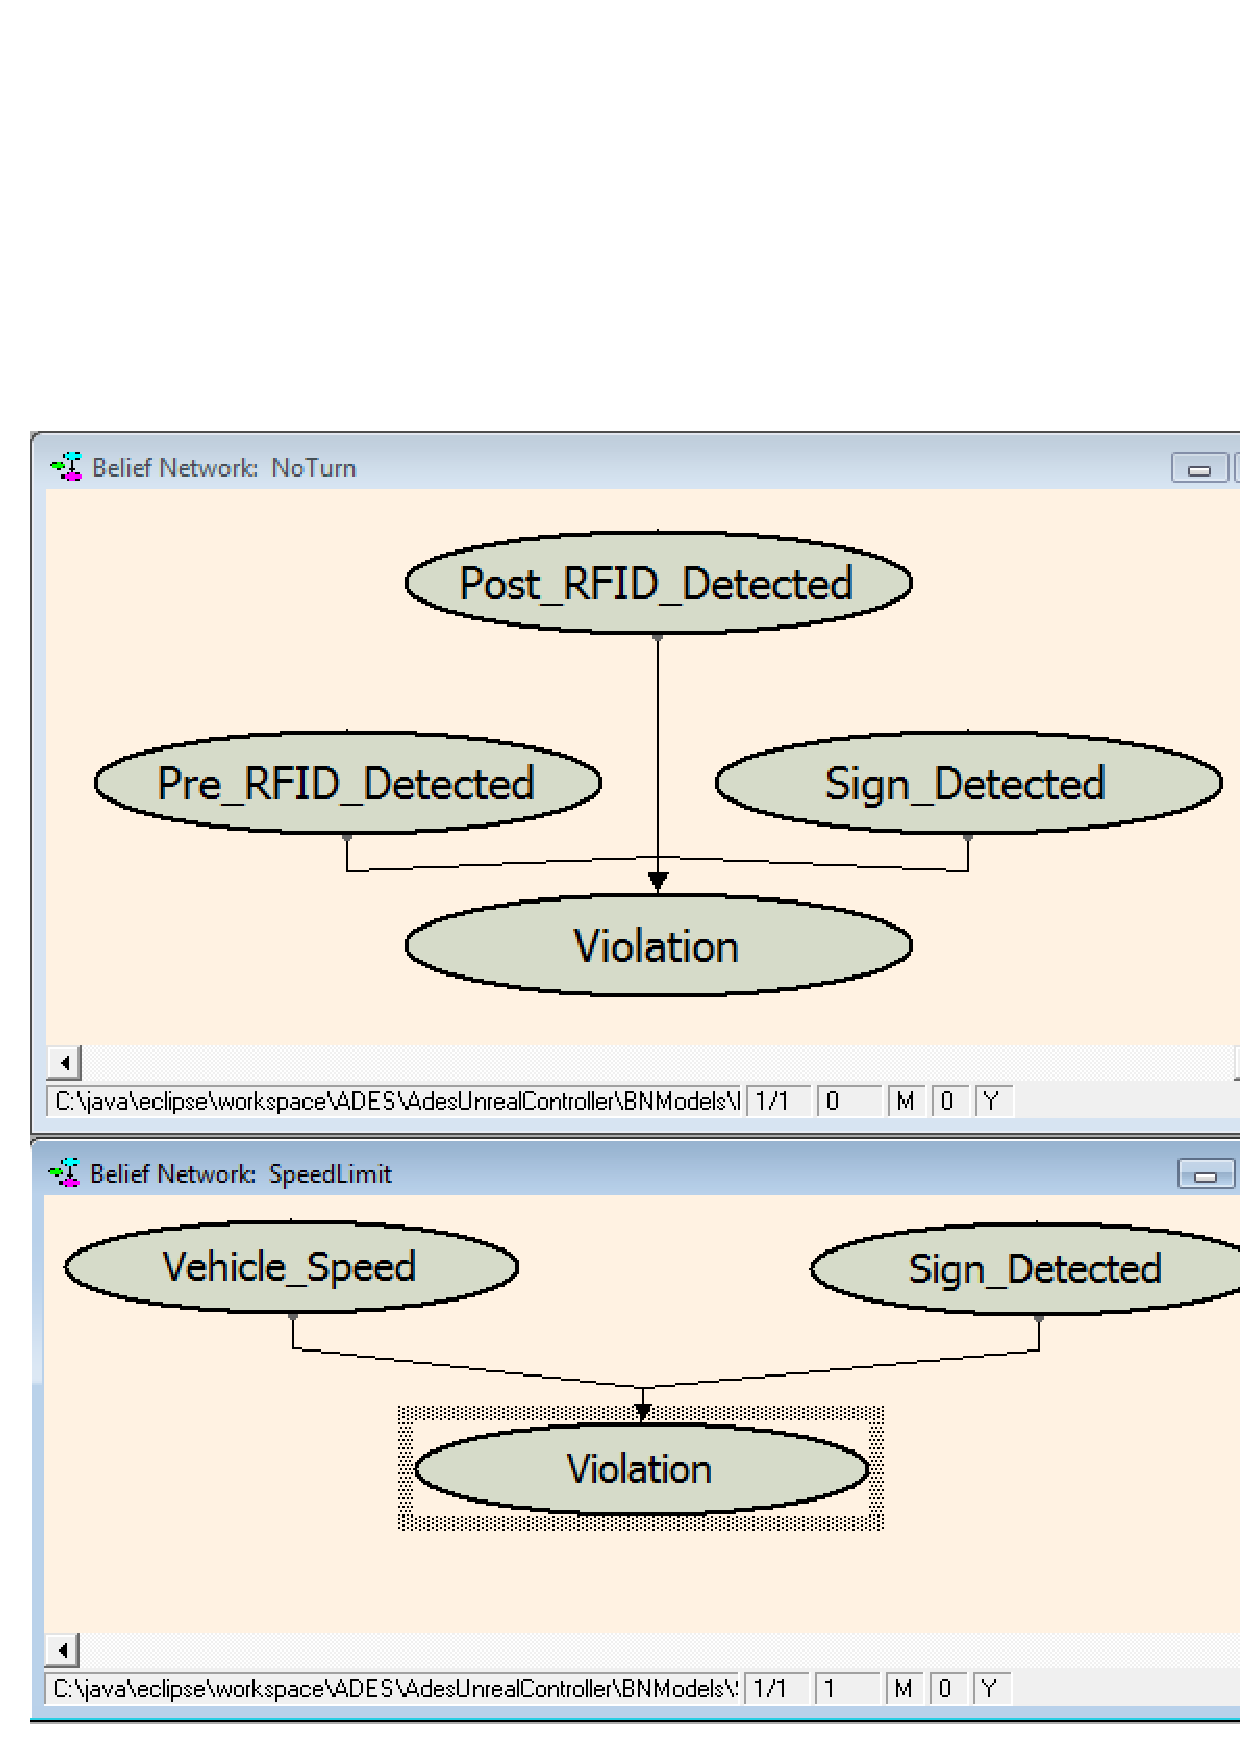
\includegraphics[scale=0.3]{img/bn}
      \caption{Belief Networks for Directional Restrictions and Speed Limitations.}
      \label{fig:bn}
\end{figure}

The $violation$ node in both networks have the same state values which are $yes$ and $no$. However, the $sign\_detected$ node has different states in each network. In the speed limitation network, the states of the $sign\_detected$ node are 30, 50, and 90 km/h signs. The $velocity$ node also has similar state values for representing the vehicle speed. On the other hand, in the directional limitations network, the $sign\_detected$ node has $no\_turn\_left$, $no\_turn\_right$, $no\_u\_turn$, and $none$ states. The states for the RFID related nodes are the same for this network.

The probability distributions of the conditionally independent nodes are assigned by the $assertFact$ function described in the expert system interface. For example, if a control RFID for no left turning restriction is sensed with a probability of $0.9$, the probability value of the $no\_turn\_left$ state becomes $0.9$ for the $post\_RFID\_detected$ node. The remaining $0.1$ is shared equally by the other three states ($no\_turn\_right$, $no\_u\_turn$, and $none$).

Different from other nodes, the probabilities of the violation node is entered to the system by the human expert during the network design as shown in Figure \ref{fig:prob}.

\begin{figure}[thb]
      \centering
      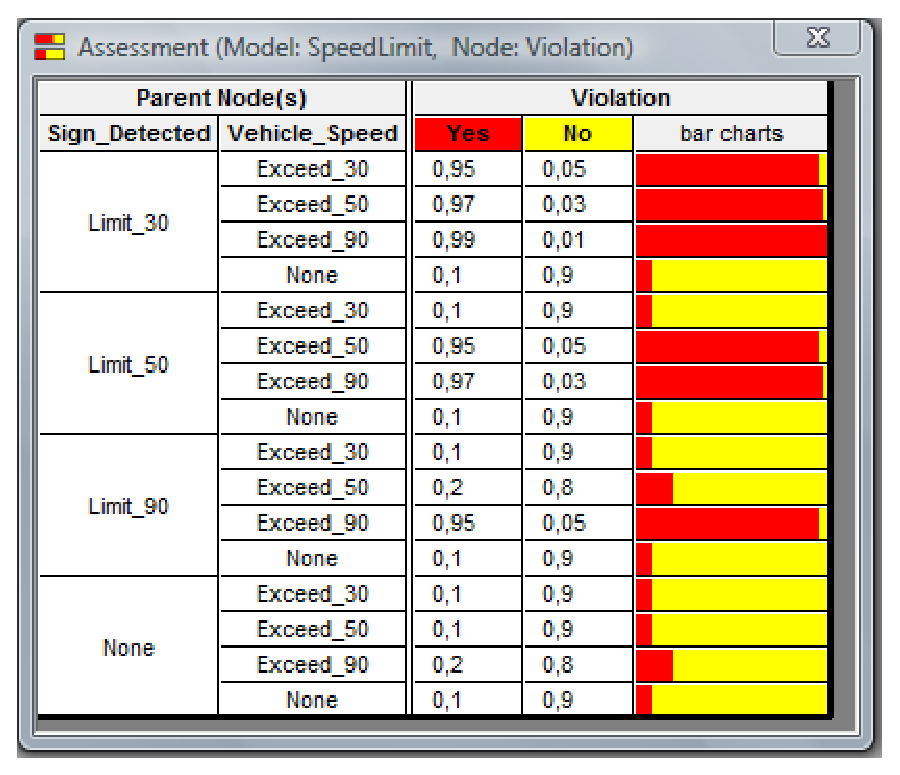
\includegraphics[scale=0.5]{img/prob}
      \caption{Belief Networks for and Speed Limitations.}
      \label{fig:prob}
\end{figure}

The probability distribution of the violation node of the belief network for the directional limitations is another table with 64 rows. The structure of the values are similar to the speed violation network, therefore this table is not presented here.

%%%%%%%%%%%%%%%%%%%%%%%%%%%%%%%%%%%%%%%%%%%%%%%%%%%%%%%%%%%%%%%%%%%%%%%%%%%%%%%%
\section{EXPERIMENTAL RESULTS}
\label{sec:experimental}

Although the ADES project targets the real physical environment, the development process can be accelerated by the use of a simulation environment. Our choice for the simulation engine is the \textit{Unreal Engine} which provides both the physics engine and the renderer ~\cite{games2006unreal}. The capabilities of this engine makes it a favorite tool for both robotics researchers and game developers. In addition to the core simulation engine, we also used \textit{USARSim} which is an \textit{Unreal Engine} expansion for urban search and rescue (USAR) robots and environments. \textit{USARSim} also provides the \textit{USARDeathMatch} game type which enables the \textit{BotServer}. The \textit{BotServer} opens a communication channel between the \textit{Unreal Engine} and the outside world. Custom objects derived from \textit{pawn} class can be initiated from remote controlling applications by connecting to this server. \textit{USARSim} also provides its own communication protocol. The details of this protocol can be found in the \textit{USARSim} manual \cite{carpin2007usarsim}.  We used the \textit{Sedan} class provided as an \textit{USARSim} model as our vehicle which is shown in Figure \ref{fig:Sedan}.

\begin{figure}[ht]
\begin{center}
\includegraphics[scale=0.25]{img/Sedan}
\caption{The Sedan in the ADES Unreal world.}
\label{fig:Sedan}
\end{center}
\end{figure}

The simulation environment requires a map where the vehicle can cruise on. This map is prepared using the level editor of the \textit{Unreal Engine}. The \textit{ADES Unreal Controller} application acts as an \textit{Unreal} client which connects to the \textit{Unreal Engine}. The engine runs a \textit{USARDeathMatch game} on the prepared map. The vehicle can be controlled by using the \textit{ADES Unreal Controller} application as shown in Fig. \ref{fig:ADESController}. Moreover, the inputs and the outputs of the expert systems can also be followed by using this application.

\begin{figure}[ht]
\begin{center}
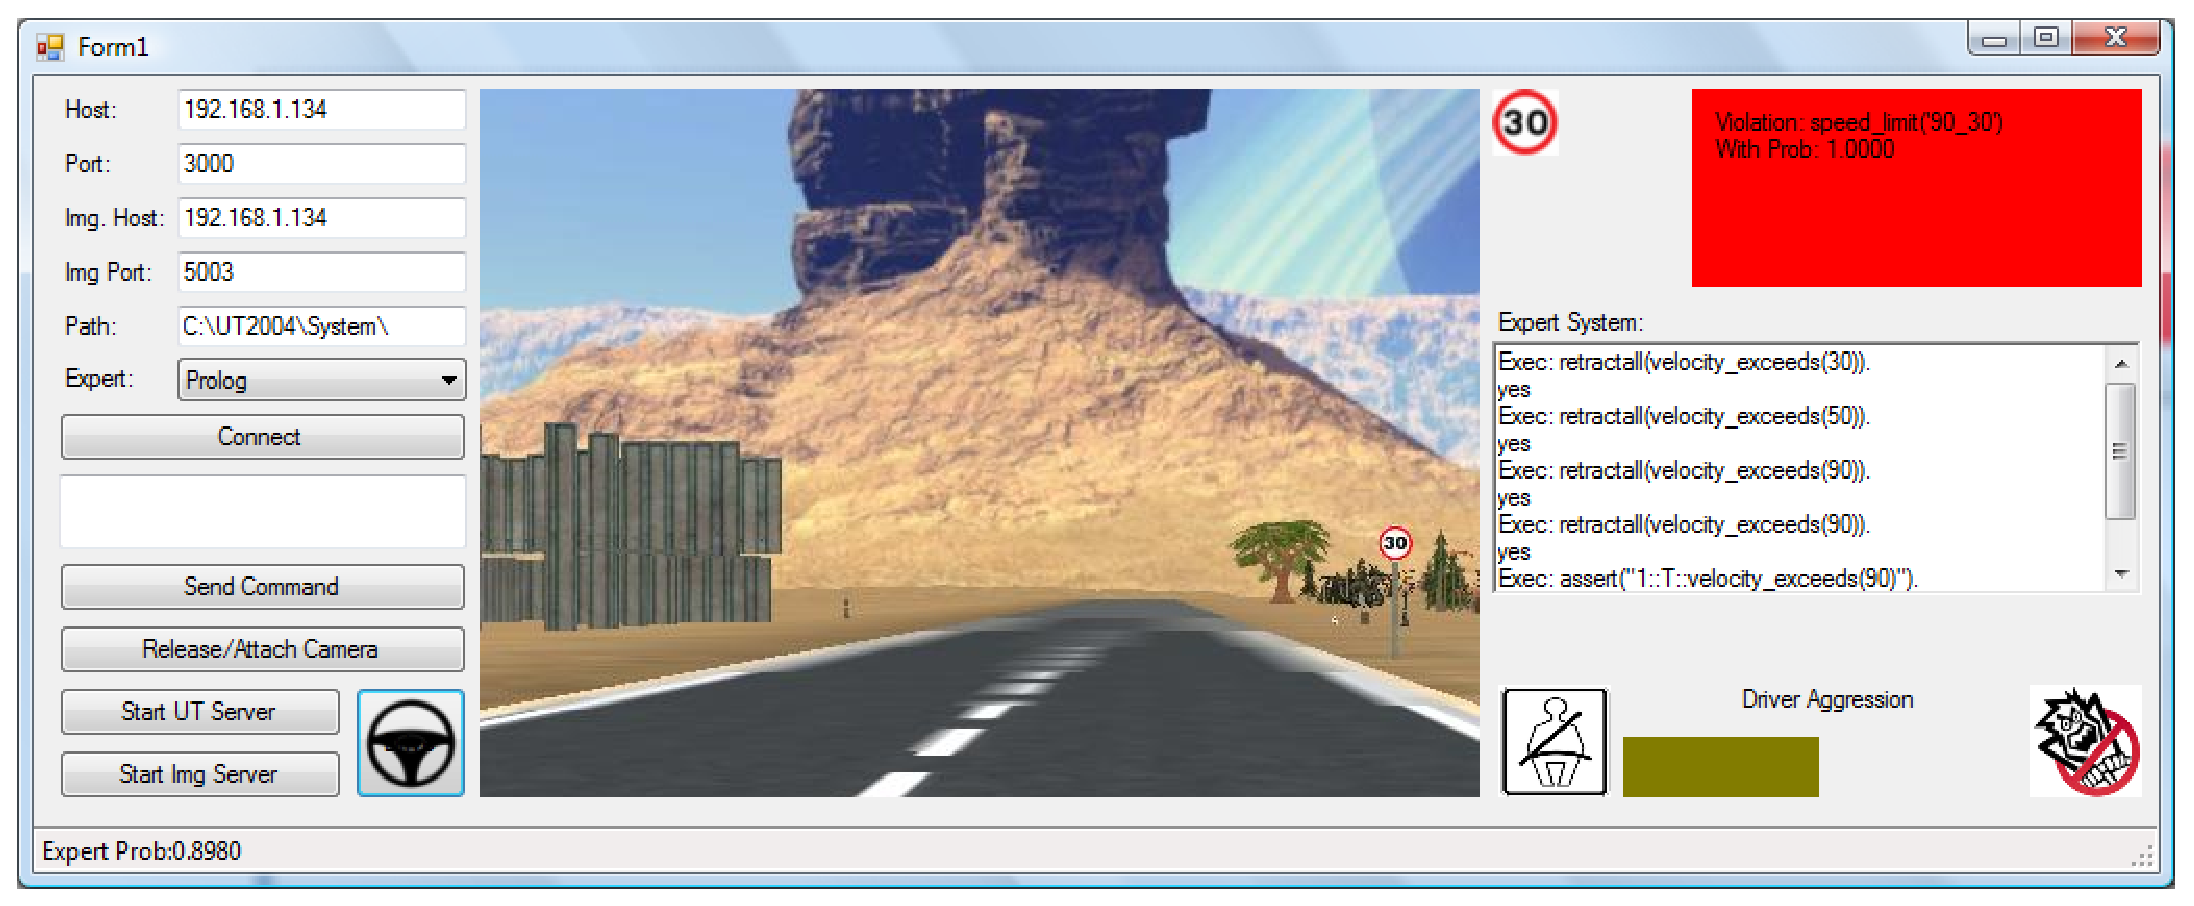
\includegraphics[scale=0.22]{img/ADESController}
\caption{The ADES Unreal Controller.}
\label{fig:ADESController}
\end{center}
\end{figure}

The sample run contains a violation condition for the 30 km/h sign and a violation for a no turning left condition. 

For the \textit{Prolog} inference engine, the underlying system is developed based on the \textit{Prolog} engine \textit{CSharp Prolog} \cite{pool09}. The inference outputs of the \textit{Prolog} expert system for these sample runs are as given in Fig. \ref{fig:InfSpeed} and Fig. \ref{fig:InfDriection}.

\begin{figure}[thb]
      \centering
\begin{mylisting}

\begin{verbatim}
Exec: retractall(sign_detected(speed_limit,30)).
yes
Exec: assert("0.9963::sign_detected(speed_limit,30)").
yes
Exec: retractall(velocity_exceeds(30)).
yes
Exec: retractall(velocity_exceeds(50)).
yes
Exec: retractall(velocity_exceeds(90)).
yes
Exec: retractall(velocity_exceeds(50)).
yes
Exec: assert("1::velocity_exceeds(50)").
yes
Exec: violation(V,A,P).
Prob for this answer:0.9963

P = 0.9963
V = speed_limit
A = '50_30'
\end{verbatim}
\end{mylisting}
      \caption{\textit{Prolog} Inference Output for Speed Limitation}
      \label{fig:InfSpeed}
\end{figure}


\begin{figure}[thb]
      \centering
\begin{mylisting}

\begin{verbatim}
Exec: retractall(sign_detected(no_turn_left)).
yes
Exec: assert("0.9999::sign_detected(no_turn_left)").
yes
Exec: retractall(rfid_detected(pre,no_turn_left)).
yes
Exec: assert("1::T::rfid_detected(pre,no_turn_left)").
yes
Exec: retractall(rfid_detected(post,no_turn_left)).
yes
Exec: assert("1::T::rfid_detected(post,no_turn_left)").
yes
Exec: violation(V,A,P).
Prob for this answer:0.9999

P = 0.999830009331709
V = no_turn_left
A = "N/A"

\end{verbatim}
\end{mylisting}
      \caption{\textit{Prolog} Inference Output for Directional Limitation}
      \label{fig:InfDriection}
\end{figure}

In both cases the expert system decides that the driver makes the related violation according to the asserted facts. The lifetime of the facts are replaced by the default value denoted as $T$. This means that these RFID readings will be available as facts for the next $45$ seconds.

For the belief network implementation, the \textit{Microsoft Bayesian Network Editor} (MSBNx), which is a \textit{Microsoft Windows} library for creating and evaluating Bayesian Networks \cite{kadie2001msbnx}, is used. It can be used as a standalone modeling and inference application, or the run-time components which provide Bayesian reasoning services can be integrated to custom applications. The graphical interface for developing BN graphs can be used in both cases. The resulting BN files can be consulted by the custom application during run-time. The inference results of the belief networks for the same samples runs are as given in Fig. \ref{fig:BNSpeed} and Fig. \ref{fig:BNDirection}.

\begin{figure}[thb]
      \centering
		   \begin{mylisting}

\begin{verbatim}
SpeedLimit:Sign_Detected()->(0.9963,0.0012,0.0012,0.0012)
SpeedLimit:Vehicle_Speed()->(0,0,1,0)
SpeedLimit violation belief 0.9890
\end{verbatim}
\end{mylisting}
      \caption{Belief Network Inference Output for Speed Limitation}
      \label{fig:BNSpeed}
\end{figure}

\begin{figure}[thb]
      \centering
		   \begin{mylisting}
\begin{verbatim}
NoTurn:Sign_Detected()->(0.9999,3e-005,3e-005,3e-005)
NoTurn:Pre_RFID_Detected()->(1,0,0,0)
NoTurn:Post_RFID_Detected()->(1,0,0,0)
NoTurn violation belief 0.8999
\end{verbatim}
\end{mylisting}
      \caption{Belief Network Output for Directional Limitation}
      \label{fig:BNDirection}
\end{figure}

The values in the parentheses are the probabilities assigned for each state for the node with the displayed name. For example, in the directional restriction inference case in Fig. \ref{fig:BNDirection},  the probability of the $no\_left\_turn$ state for the $Sign\_Detected$ node is $0.9963$. Similarly the pre and post RFID detection nodes have a perfect sensing value for their $no\_left\_turn$ states. However, different from the previous method, the probability of the violation is not simply the multiplication of the probabilities of the selected state probabilities. The probability distribution of the violation node should also be considered. For example, in the speed limit inference case, the $Sign\_Detected$ node has the highest probability value for $30~km/h$ sign which is $0.9963$. In addition, the $Vehicle\_Speed$ node states that the velocity of the vehicle exceeds $90~km/h$ with the probability of $1$. The probability of the violation is calculated from the following equation,


\begin{equation}
	p_{v} = \sum_{d\in{Sign\_Detected},s\in{Vehicle\_Speed}}p_{d} \times p_{s} \times vp(d,s)
\end{equation}


\noindent
where $d$ and $s$ are the state probabilities for  $Sign\_Detected$ and $Vehicle\_Speed$ nodes. $vp$ denotes the probability values for violation node which can be found from Figure \ref{fig:prob}. For this particular case  $p_{v}$ is calculated as:

\begin{eqnarray*}
p_{v} &=& 0.9963 \times 1 \times 0.99 \\
& & + 0.0012 \times 1 \times 0.97  \\
& & + 0.0012 \times 1 \times 0.95  \\
& & + 0.0012 \times 1 \times 0.2  \\
p_{v} &=& 0.9890
\end{eqnarray*}

\noindent
Note that the arguments which are zero due to the $vs$ multiplicand are not shown in the equation above. 

%%%%%%%%%%%%%%%%%%%%%%%%%%%%%%%%%%%%%%%%%%%%%%%%%%%%%%%%%%%%%%%%%%%%%%%%%%%%%%%%
\section{DISCUSSION AND CONCLUSIONS}
\label{sec:conc}

In this study we propose two expert system designs for evaluating the driver violations in the ADES project. The implemented expert systems are based on \textit{Prolog} and Belief Networks. The properties of these methods are compared on Table \ref{tab1} and \ref{tab2}.

\begin{table}[!ht]
\caption{Properties of expert system models.}
\centering
{\scriptsize
\begin{tabular}{|p{13mm}|p{30mm}|p{30mm}|}
\hline
 & {\bf Probabilistic Model} & {\bf Rule Based Model} \\
\hline
{\bf Knowledge Base} & Probabilistic Structure,  Facts & Rules, Facts \\
\hline
{\bf Inference Engine} & Conditional probability evaluation (Bayes theorem) & Backward chaining, Forward chaining \\
\hline
{\bf Explanation Subsystem} & Based on conditional probabilities & Based on triggered rules \\
\hline
{\bf Learning Subsystem} & Change in probabilistic structure and probabilities & Adding, removing rules \\
\hline
\end{tabular}
}
\label{tab1}
\end{table}

\begin{table}[!ht]
\caption{Comparison of expert systems models.}
\centering
{\scriptsize
\begin{tabular}{|p{13mm}|p{30mm}|p{30mm}|}
\hline
 & {\bf Probabilistic Model} & {\bf Rule Based Model} \\
\hline
{\bf Advantages} & Easy learning, Easy probability propagation & Easy explanation, Easy modification \\
\hline
{\bf Shortcomings} & High number of parameters, Detection of unnecessary rules & Performance issues, Certainty implementation \\
\hline
\end{tabular}  
}
\label{tab2}
\vskip -5pt
\end{table}

Both models have advantages and disadvantages. The probabilistic model provides a proper handling of uncertainty with easy learning capabilities. Statistical information can be used directly to form a probabilistic model. However, relatively high number of parameters even in a small model makes the model more complicated both for understanding and management. On the other hand, the rule based systems are easier to maintain. However, this advantage usually causes performance issues for complex problems where extensive rule chaining is required.

Another issue is the retraction of the facts from the system. The retraction process is as important as the assertion of the facts since invalidated facts can cause misleading decisions. Although the \textit{Prolog} based expert system provides a lifetime limit for the facts, additional controls should be considered for asserted facts.

The threshold used by the expert system is defined by the human expert. However, our implementation slightly changes this threshold according to the previous actions of the driver. In other words, the expert system favors a driver who drives safely by increasing the threshold value for the violation probability. Similarly, the threshold is decreased to a predefined level for faulty drivers.

A simulated environment is generated in this study to present the problem and introduce two possible expert system implementations for the solution. Other expert systems with more complex rules robust to real life data can be developed as a future work.

\bibliographystyle{ieeetr}
\bibliography{ades_es}	

\end{document}